\documentclass[../mit-general-chemistry.tex]{subfiles}
\begin{document}

\chapter{Transition metals}


The transition metals are the elements of the $d$ block of the
periodic system.

The study of transition metals is in a large part part of inorganic
chemistry, more specific bioinorganic chemistry. Here a big field is
tracking occurrence and functions of metal ions in biological
systems. These are added or removed from proteins to do ``cool
things''.

Some of the functions of transition metals in the body are
\begin{itemize}
\item Global cycling of nitrogen, carbon and hydrogen
\item Radical reactions
\item Biosynthesis of vitamins
\item Biosynthesis of deoxynucleotides
\end{itemize}




\section{Coordination complexes}



A key feature of the transition metals are their ability to form
complexes with small molecules and ions.

Positive metal ions can attract electron densities, usually a lone
pair from another molecule or atom to form a {\em coordination
  complex} or {\em coordination compounds}. Donor atoms are called
{\em ligands} (by Lewis). Ligands are Lewis bases --- they donate
electrons. Ligands typically donate one lone pair of electrons. This
makes the central atom or ion of the complex a Lewis acid as it
accepts electrons from the ligands.


Some examples of coordination complexes are found in biochemistry and
are involved in essential functions in the body.

\begin{itemize}
\item
  Hemoglobin carries oxygen to the cells of the body through the blood
  and carbon dioxide back to the lungs. It is an iron complex that
  carries oxygen and carbon dioxide through the vascular system.
\item
  Cytochrome consists of an iron complex that transfer electrons
  within the cell.
\item
  Many enzymes are coordination complexes with central atoms of iron,
  copper, zinc and molybdenum. They are catalysts in reactions
  throughout the body.
\end{itemize}

Ligands are often compounds of oxygen, nitrogen, carbon and hydrogen.

\begin{hfigure}
  \hspace*{\fill}
  \chemfig{\lewis{4:,N}O2^{-}}
  \hfill%
  \hfill%
  \chemfig{\lewis{4:,O}CO2^{2-}}
  \hfill%
  \chemfig{\lewis{4:,C}N^{-}}
  \hfill%
  \chemfig{\lewis{4:,S}CN^{-}}
  \hfill%
  \chemfig{\lewis{4:,N}CS^{-}}
  \hspace*{\fill}

  \hspace*{\fill}
  \chemfig{\lewis{4:,O}H^{-}}
  \hfill%
  \hfill%
  \chemfig{\lewis{4:,O}H2}
  \hfill%
  \chemfig{\lewis{4:,N}H3}
  \hfill%
  \chemfig{\lewis{4:,C}O}
  \hfill%
  \chemfig{\lewis{4:,N}O^{+}}
  \hspace*{\fill}
  \caption{Examples of ligands.}
\end{hfigure}


A key feature of the transition metals is their ability to form
complexes with small molecules and ions. The complexes are formed as
positive metal ions attract electron densities, usually a lone pair of
electrons, from the molecule or ion.

Ligands act as Lewis bases as they donate electron pairs. The
transition metal act as a Lewis acid as it accepts electrons. Common
transition metals are \ce{Ti, Cr, Mn, Fe, Co, Ni, Sn, Ir, Pt}. {\em
  Coordination complexes} are transition metals surrounded by ligands.



\begin{hfigure}
  \newcommand\bondlength{1.5}
  \begin{equation*}
    \left[~\chemfig{Co
        (-[:90,\bondlength]\lewis{4:,N}H3)
        (<:[:150,\bondlength]H3\lewis{2:,N})
        (<[:210,\bondlength]H3\lewis{6:,N})
        (-[:270,\bondlength]\lewis{4:,N}H3)
        (<[:330,\bondlength]\lewis{6:,N}H3)
        (<:[:30,\bondlength]\lewis{2:,N}H3)}
      ~\right]^{3+}
  \end{equation*}

  \caption{Examples of a coordination complex (\ce{Co(NH3)6}). The
    cobalt atom bonds with the nitrogen atoms and their free electron
    pairs. The cobalt atom acts as a Lewis acid. The complex has three
    \ce{Cl^-} {\em counter ions}.}
\end{hfigure}



Sometimes the coordination complexes are charged. They are then
associated with {\em counter ions}.

The coordination complex above can be described with the notation
\begin{equation}
  \ce{[Co(NH3)6]^{3+} 3Cl^- -> [Co(NH3)6]Cl3}
\end{equation}

for three chloride counter ions.

\paragraphbreak

The {\em coordination number} (\coordinationnumber) of a coordination
complex is the number of ligands in the coordination complex. In the
example above, the coordination number is $\coordinationnumber = 6$ as
the cobalt atom is connected to six \ce{NH3} ligands. Coordination
numbers usually lie between two and twelve. Six ligands is the most
common coordination number of coordination complexes.


The coordination number is associated with geometric shapes of the
coordination complex. The \ce{CO(NH3)6} complex above,
$\coordinationnumber = 6$, is a molecule with an octahedral shape.

%\newcolumntype{R}{>{\raggedleft\arraybackslash}X}
%\usepackage{ragged2e} % for "\RaggedRight" macro  
%\newcolumntype{P}[1]{>{\RaggedRight\arraybackslash}p{#1}}

\begin{htable}
  \begin{center}
    \begin{tabularx}{.67\textwidth}{p{2cm}X}
      Coordination number & Geometric shape \\
      \midrule
      6 & octahedral (and triagonal prismatic) \\
      5 & triagonal bipyramidal or square pyramidal \\
      4 & square planar, tetrahedral or seesaw \\
      3 & triagonal planar \\
      2 & linear \\
    \end{tabularx}
  \end{center}
  \caption{Geometric shapes associated with coordination numbers.}
\end{htable}



\subsection{Chelate effect}

Denticity refers to the number of donor groups in a single ligand that
bind to a central atom in a coordination complex. In many cases, only
one atom in the ligand binds to the metal, so the denticity equals
one, and the ligand is said to be monodentate (sometimes called
unidentate). Ligands with more than one bonded atom are called
polydentate or multidentate. The word denticity is derived from
dentis, the Latin word for tooth. The ligand is thought of as biting
the metal at one or more linkage points. The denticity of a ligand is
described with the Greek letter $\kappa$ ('kappa').


{\em Chelation} is a type of bonding of ions and molecules to metal
ions. It involves the formation or presence of two or more separate
coordinate bonds between a polydentate (multiple bonded) ligand and a
single central atom. Usually these ligands are organic compounds, and
are called chelants, chelators, chelating agents, or sequestering
agents.


If a ligand binds to the central atom with two points of attachment
it is said to be {\em bidentate}. Subsequent types of chelants are
said to be {\em tridentate}, {\em tetradentate}, {\em hexadentate} and
so on. These examples are seen in the table below.

\begin{inlinetable}{cl}
  $\kappa$ & name \\
  \midrule
  2 & bidentate \\
  3 & tridentate \\
  4 & tetradentate \\
  6 & hexadentate \\
\end{inlinetable}


Metal chelates are unusually stable. This is in part due to the fact
that these bonds are favoured over bonds between the metal ions and
non-chelating ligands \blockquote[\cite{courselectures}]{...due to the
  favorable entropic factor accompanying release of non-chelating
  agents (usually water) from the coordination sphere.}


Sequestering agents are chelating agents that are used to remove
unwanted metal ions. In medicine sequestering agents are used to
selectively remove toxic metal ions (e.g. \ce{Hg^2+} and \ce{Pb^2+})
while leaving biologically important metals.

\begin{example}
  Vitamin \ce{B12} is an example of a coordination complex. The cobalt
  central atom has three ligands connected to it.

  Cobalt is coordinated by a planar tetradental ligand, a {\em corrin
    ring system}. This is a chelate as it is bound to the cobalt atom
  through four atoms -- it is tetradentate.

  It is also coordinate by an upper axial ligand (5'deoxysdenosine)
  and a lower axial ligand (dimethylbenzimidazole).

  The corrin ring around the central atom makes for a square planar
  geometry and the two axial ligands give the geometry of the entire
  molecule to an octagonal shape (two four-sided pyramids with the
  base against each other).

  Vitamin \ce{B12} is a fairly complex vitamin. It is actually one of
  the most complex vitamins that is known. It's structure was first
  determined in the 1940s by the British x-ray crystallographer
  Dorothy Crowfoot Hodgkin and is a pioneering work with that
  technique.
\end{example}

\begin{example}
  Another example of a chelate is ethylenediamine tertraacetic acid
  (EDTA).

  The molecule contains six oxygen and nitrogen atoms with lone
  electron pairs that can be found to bond (be donated) to coordinate
  a metal ion and form a coordination complex.

  A coordination complex of EDTA and a central metal atom is, thus, a
  hexadentate chelate and the shape of the complex is octahedral.

  When EDTA coordinates metal atoms in this way, the coordination
  complex is very stable, due to the chelate effect. This give such
  compounds important uses such as removing metals from solutions. One
  such use, that is very important, is neutralizing lead poisoning.

  EDTA is added to food to prevent bacteria and fungi to grow on
  them. As EDTA binds to the metals in the food, it prevents the
  metals to be digested by the microbes. Metals are essential to
  microbes and humans and so this decreases growth of microbes on the
  products.

  EDTA is also used in bathroom cleaners as bath scum contains chelate
  calcium ions.
\end{example}


\subsection{Isomers}

Geometric isomers of coordination complexes can have very different
properties. This can be very important in biological systems.

$[\ce{Pt(NH3)2Cl2}]$ has two geometric isomers.

\begin{hfigure}
  \newcommand\bondlength{1.5}
  \hspace*{\fill}
  \chemname{
    \chemfig{Pt
      (<:[:30,\bondlength]Cl)
      (<:[:150,\bondlength]H3N)
      (<[:210,\bondlength]H3N)
      (<[:330,\bondlength]Cl)
    }
  }{cisplatin}
  \hfill%
  \chemname{
    \chemfig{Pt
      (<:[:30,\bondlength]Cl)
      (<:[:150,\bondlength]H3N)
      (<[:210,\bondlength]Cl)
      (<[:330,\bondlength]NH3)
    }
  }{transplatin}
  \hspace*{\fill}

  \caption{Isomers of $[\ce{Pt(NH3)2Cl2}]$.}
\end{hfigure}

Cisplatin is a known, potent drug for treatment of cancer, whereas
transplatin has no known (medical) use. The difference is due to the
placement of the ammonia groups (\ce{NH3}) of the complex even though the
summation formulas are identical.

Research has shown that cisplatin can bind to DNA, whereas transplatin
can not, and this is the distinction between the two compounds. As
cisplatin binds to the DNA of the cancer cell, this is what actually
kills the cell as it inhibits the transcription of the DNA.

Thus geometric isomers can have different properties, even though they
have the same composition (i.e. summation formula), due to their
geometric configurations.

\paragraphbreak

{\em Optical isomers} (enantiomers) are non-superimposable mirror
images of each other (fig). A complex that is not identical to it's
mirror image is called a {\em chiral} complex.

\begin{hfigure}
  \newcommand\bondlength{1.5}
  \hspace*{\fill}
  \chemfig{Co
    (<:[:30,\bondlength]Cl)
    (-[:90,\bondlength]NH3)
    (<:[:150,\bondlength]H3N)
    (<[:210,\bondlength]H2O)
    (-[:270,\bondlength]Cl)
    (<[:330,\bondlength]OH2)
  }
  \hfill%
  \chemfig{Co
    (<:[:30,\bondlength]NH3)
    (-[:90,\bondlength]NH3)
    (<:[:150,\bondlength]Cl)
    (<[:210,\bondlength]H2O)
    (-[:270,\bondlength]Cl)
    (<[:330,\bondlength]OH2)
  }
  \hspace*{\fill}

  \caption{Examples of {\em optical isomers}. The asymmetry of the
    ammonia and chloride groups make the two structures
    non-superimposable.}
\end{hfigure}

Chiral molecules have different properties in {\em chiral
  environments}.


\begin{remark}
  My understanding is that it is an environment in which, when the
  isomers interact with the environment, the two enantiomers can be
  distinguished.
  
  That's exactly right. Some examples of chiral environments that
  could be created in a lab would include

  \begin{itemize}
  \item Running a reaction in a chiral solvent
  \item Running a reaction in a chiral cavity
  \item
    Running a reaction with a chiral reagent
  \item
    Running a photochemical reaction with a polarized light source
  \item
    Carrying out a reaction on a surface to which chiral molecules
    have been attached (certain clays have this property)
  \end{itemize}

  All of these items are like a glove, and each enantiomer will fit
  differently. This different "fit" leads to transition states of
  different energy as each enantiomer moves along the reaction
  coordinate towards the product(s).

  	
  If you run a reaction that can produce 2 enantiomers in a chiral
  environment, then one enantiomer will be preferentially
  produced. Because in the chiral environment the two possible
  transition states will be diastereomeric (e.g. of different
  energy). If the chiral environment is "strong" enough then one
  enantiomer may be produced to the exclusion of the other
  enantiomer. I'm not sure I understand the second part of your comment,
  but both enantiomers and the transition states leading to them are
  diasteromeric in a chiral environment, so the transition states will
  have different energies leading to the preferred formation of one
  enantiomer over the other.
\end{remark}








\subsection{$d$-orbitals}



The transition metals are mainly residing in the $d$ block of the
periodic table. This means that we have to start consider electrons of
the $d$ orbitals of the elements.



There are five $d$ orbitals: $d_{xy}$, $d_{xz}$, $d_{yz}$, $d_{z^2}$
and $d_{x^2-y^2}$. Four of the five d-orbitals look similar, each with
four pear-shaped lobes, each lobe tangent at right angles to two
others, and the centers of all four lying in one plane. Three of these
planes are the xy-, xz-, and yz-planes —- the lobes are between the
pairs of primary axes (\ang{45}) -— and the fourth has the centres
along the x and y axes themselves. The fifth and final d-orbital
consists of three regions of high probability density: a torus with
two pear-shaped regions placed symmetrically on its z axis. The
overall total of 18 directional lobes point in every primary axis
direction and between every pair.



\begin{hfigure}
  \begin{center}
    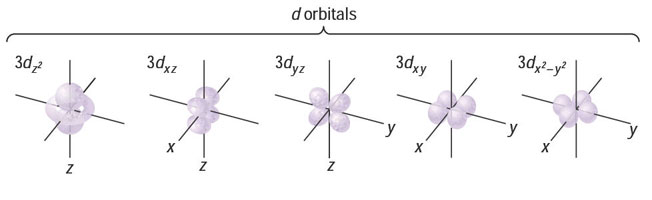
\includegraphics[width=\textwidth]{d-orbitals}
  \end{center}
  \caption{An illustration of the five $d$ orbitals.}
\end{hfigure}



We can calculate the electrons of the $d$ orbitals of a metal in a
coordination complex from
\begin{equation}
  n_{d-\text{electrons}} = \text{group number} - \text{oxidation state}
\end{equation}


\begin{example}
  We consider the complex from earlier, $\ce{[Co(NH3)6]^{3+}}$. To
  calculate the number of electrons in the $d$ orbital of the cobalt
  atom we first see that the ammonia groups have an oxidation state of
  zero since hydrogen has an oxidation state of $+1$, nitrogen must have
  an oxidation state of $-3$. This tell us that the oxidation state of
  cobalt must be $+3$ -- the charge of the complex.

  The group number of cobalt is nine (9) so the number of electrons in
  the $d$ orbital of cobalt in this complex is
  \begin{equation*}
    n = 9 - 3 = 6~\text{electrons}
  \end{equation*}

  This makes the combalt of this complex a ``$d^6$ system''.
\end{example}

We look at some other examples.

\begin{example}
  Consider \ce{[Ni(CO)4]}.

  The oxidation state of oxygen is $2$ in most compounds. This makes
  the oxidation state of carbon $-2$ since carbon monoxide molecules
  are uncharged. Since the complex also is uncharged, this makes the
  oxidation state of nickel equal to zero.

  Nickel belongs to group ten of the periodic table and
  \begin{equation*}
    n = 10 - 0
  \end{equation*}
  which makes \ce{[Ni(CO)4]} a $d^{10}$ system.
\end{example}

\begin{example}
  Consider \ce{[Co(H2O)2(NH3)Cl]^-}.

  Since ammonia and water are uncharged molecules we do not need to
  consider them in calculating the oxidation state of cobalt in this
  complex. We conclude that the oxidation state of each of the three
  chlorine atoms is $-1$ since chlorine usually have an oxidation
  state of $-1$ in compounds not including oxygen or fluoride. We also
  note that the charge of the complex is (also) $-1$.

  We can now calculate the oxidation state of cobalt (in this complex)
  as
  \begin{equation*}
    \text{ox}_{\ce{Co}}
    = \underset{\text{ion charge}}{(-1)}
    - \underset{\text{ox(\ce{Cl})}}{3\cdot(-1)} = 2
  \end{equation*}

  Since cobalt belong to group $9$ of the periodic table we can
  calculate the number of electrons of the $d$ orbitals ($n_d$) of
  cobalt as
  \begin{equation*}
    n_d = 9 - 2 = 7
  \end{equation*}
  which makes \ce{[Co(H2O)2(NH3)Cl]^-} a $d^7$ system.
\end{example}







\section{Crystal field theory}




{\em Crystal field theory} and {\em Ligand field theory} was developed
to explain the special properties of coordination complexes of
transition metals.

A metal ion, with a given oxidation state, when placed in a
coordination sphere, defined by a set of ligands, alter its electron
configuration to the electron configuration of that of a free metal
ion.

Crystal field theory is an electrostatic approach, used to describe
the split in metal d-orbital energies within an octahedral
environment. It provides an approximate description of the electronic
energy levels often responsible for the ultraviolet and visible
spectra of coordination complexes, but it does not describe
metal–ligand bonding.
\autocite[363]{miessler2014}

Ligand field theory is a description of bonding in terms of the
interactions between metal and ligand frontier orbitals to form
molecular orbitals. It uses some crystal field theory terminology but
focuses on orbital interactions rather than attractions between ions.
\autocite[363]{miessler2014}




\subsubsection{Crystal field theory}


Crystal field theory considers the ligands as negative point charges
and the repulsion between these and the $d$ orbitals of the transition
metal species.



\begin{hfigure}
  \newcommand\bondlength{1.5}
  \hspace*{\fill}
  \chemfig{M^n+
    (<:[:45,\bondlength]L^{-})
    (-[:90,\bondlength]L^{-})
    (-[:180,\bondlength]L^{-})
    (<[:225,\bondlength]L^{-})
    (-[:270,\bondlength]L^{-})
    (-[:0,\bondlength]L^{-})
  }
  \hfill
  \begin{tikzpicture}[thick,scale=2.5]
    \def\opacity{0.6}
    \coordinate (A1) at (0,0);
    \coordinate (A2) at (0.6,0.2);
    \coordinate (A3) at (1,0);
    \coordinate (A4) at (0.4,-0.2);
    \coordinate (B1) at (0.5,0.5);
    \coordinate (B2) at (0.5,-0.5);
    
    \begin{scope}[thick,dashed,,opacity=0.6]
      \draw (A1) -- (A2) -- (A3);
      \draw (B1) -- (A2) -- (B2);
    \end{scope}
    \draw[fill=cof,opacity=\opacity] (A1) -- (A4) -- (B1);
    \draw[fill=pur,opacity=\opacity] (A1) -- (A4) -- (B2);
    \draw[fill=greeo,opacity=\opacity] (A3) -- (A4) -- (B1);
    \draw[fill=greet,opacity=\opacity] (A3) -- (A4) -- (B2);
    \draw (B1) -- (A1) -- (B2) -- (A3) --cycle;
  \end{tikzpicture}
  \hspace*{\fill}
  
  \caption{A coordination complex with four ligands. The shape of the
    molecule is obvously bipyramidal or tetrahedral.}
\end{hfigure}










\end{document}
